\subsubsection{Conservation Laws}

\paragraph{TheundefinedMethodundefinedofundefinedCharacteristics}

\subparagraph{IntegralundefinedSurface}

ConsiderundefinedtheundefinedgeneralundefinedquasilinearundefinedfirstundefinedorderundefinedPDE:
\begin{equation}
a(x,y,u)u_x + b(x,y,u)u_y = c(x,y,u)
\end{equation}
Weundefinednoteundefinedthatundefinedtheundefinedvectorundefinedfieldundefined$( -u_x, -u_y, 1)^T$undefinedwouldundefinedbeundefinedorthogonalundefinedtoundefinedtheundefinedsolutionundefined$u(x,y)$undefinedeverywhere.undefinedThereforeundefinedtheundefinedvectorundefinedfieldundefined$(a, b, c)^T$undefinedisundefinedperpendicularundefinedtoundefined$( -u_x, -u_y, 1)^T$undefinedthusundefinedmustundefinedlieundefinedinundefinedtheundefinedtangentundefinedplaneundefinedofundefined$u(x,y)$.undefinedSurfacesundefinedthatundefinedareundefinedtangentundefinedtoundefinedaundefinedvectorundefinedspaceundefinedisundefinedcalledundefined\textit{integralundefinedsurfaces},undefinedhenceundefinedtoundefinedfindundefinedtheundefinedsolutionundefinedweundefinedwantundefinedtoundefinedfindundefinedtheundefinedintegralundefinedsurfacesundefinedofundefined$u(x,y)$.

Weundefineddoundefinedthisundefinedby:

\begin{mystadmonition}{mystAmber}{MethodundefinedofundefinedCharacterisitcs}\begin{enumerate}
\item Parametrizeundefinedtheundefinedinitalundefinedconditionundefined$\Gamma(r)$
\item Findundefinedintegralundefinedcurvesundefined$\chi$undefinedstartingundefinedfromundefinedoneundefinedinstanceundefinedofundefinedtheundefinedinitialundefinedcondition(atundefinedsomeundefined$r$)undefinedbyundefinedsolvingundefinedaundefinedsystemundefinedofundefinedODE.
Concretely,undefinedsupposeundefined$\chi(s) = (x(s),y(s),z(s))$undefinedisundefinedaundefinedparametrizationundefinedofundefinedtheundefinedintegralundefinedcurves,undefinedthenundefineditundefinedmustundefinedsatisfyundefinedthat:
\begin{equation}
\begin{cases}
\frac{dx}{ds}&=a(x,y,u) \\
\frac{dy}{ds}&=b(x,y,u) \\
\frac{dz}{ds}&=c(x,y,z) \\
\end{cases}
\end{equation}
onundefinedsomeundefinedsmallundefined$|t -t_0|<\delta$.undefinedundefinedTheundefinedresultingundefinedintegralundefinedcurvesundefinedareundefinedfunctionsundefinedofundefined$r,s$undefinedwhereundefined$r$undefinedspecifiesundefinedwhereundefinedtheundefinedevolutionundefinedstartundefinedandundefined$s$undefinedspecifiesundefinedhowundefinedmuchundefinedtheundefinedintegralundefinedcurveundefinedgrowundefinedawayundefinedfromundefinedtheundefined$\Gamma$.


\item Computeundefinedtheundefinedintegralundefinedsurfaceundefinedasundefinedaundefinedcontinuousundefinedunionundefinedbyundefinedreplacingundefined$r,s$undefinedwithundefined$x,y$
\end{enumerate}

\end{mystadmonition}
\begin{mystthmexample}{ConstantundefinedWave-speedundefinedAdvection}{example-conservationlaws-1}Considerundefinedtheundefinedequationundefined$u_t+cu_x=0$undefinedwithundefinedtheundefinedinitialundefinedconditionundefined$u(t,0)=\exp( -x^2)$.undefinedWeundefinedparametrizeundefinedtheundefinedinitialundefinedconditionundefinedasundefined$(t,x,z)=(0,r,\exp( -r^2))$.undefinedFixundefined$r$,undefinedtheundefinedsystemundefinedis:
\begin{equation}
\begin{cases}
   \frac{dt}{ds}&=1 \\
   \frac{dx}{ds}&=c \\
   \frac{dz}{ds}&=0 \\
   \end{cases}
   \Longrightarrow
   \begin{cases}
   t(r,s)=s+C(r) \\
   x(r,s)=cs+D(r)\\
   z(r,s)=E(r) \\
   \end{cases}
\end{equation}
Substitutingundefinedtheundefinedinitialundefinedcondition,undefinedweundefinedget:
\begin{equation}
\begin{cases}
   t(r,s)=s \\
   x(r,s)=cs+r\\
   z(r,s)=\exp(-r^2) \\
   \end{cases}
\end{equation}
Butundefinednowundefined$r=x -cs=x -ct$undefinedhenceundefinedweundefinedgetundefinedtheundefinedsolution:
\begin{equation}
u(t,x)=\exp(-(x-ct)^2)
\end{equation}
Visualizingundefinedtheundefinedsolution:

\end{mystthmexample}
\begin{figure}[!htbp]
\centering
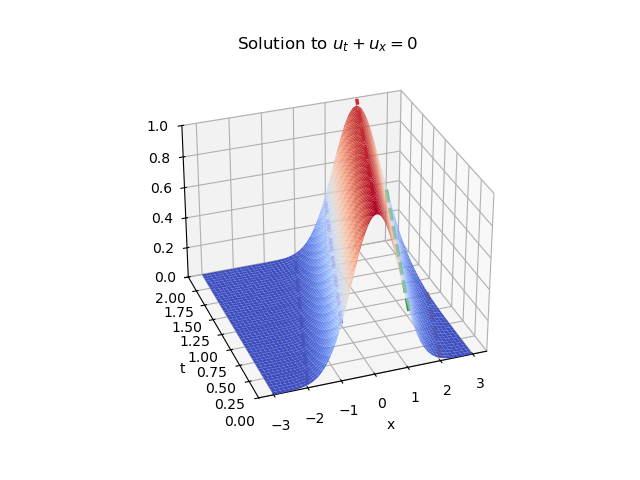
\includegraphics[width=0.7\linewidth]{files/ex1-12fb0a22df1e48f3994c66c3b0db0eda.png}
\caption*{Weundefinedshowedundefinedtheundefinedspecialundefinedcaseundefinedwhenundefined$c=1$,undefinedtheundefinedlinesundefinedareundefinedtheundefinedintegralundefinedcurvesundefinedabove.undefinedInundefinedthisundefinedspecialundefinedcaseundefinedtheundefinedvalueundefinedofundefined$z=u(x,y)$undefinedisundefinedfixedundefinedonundefinedtheundefinedcurve.}
\end{figure}

\paragraph{TheundefinedFiniteundefinedVolumeundefinedMethod}

\subparagraph{HyperbolicundefinedConservationundefinedLaw}

Forundefinedsimplicity,undefinedweundefinedconsiderundefinedtheundefinedhomogenousundefinedcase:
\begin{equation}
u_t + a(t,x)u_x = 0
\end{equation}
Ifundefinedweundefineddiscretizeundefinedtheundefinedspatialundefineddomainundefinedintoundefinedanundefinedarrayundefinedofundefinedcontiguousundefinedcellsundefinedcalledundefined\textit{controlundefinedvolumes},
weundefinedcanundefinedseeundefinedthatundefinedtheundefinedequationundefinedencapsulateundefinedaundefinedsenseundefinedofundefined\textit{conservation}.undefinedSupposeundefined$[a,b]$undefinedisundefinedaundefinedcellundefinedofundefinedinterest,undefinedintegrateundefinedtheundefinedequationundefinedbyundefinedpartsundefinedresultsundefinedinundefined:
\begin{equation}
\frac{d}{dt}\int_{a}^b u  dx = \underbrace{a(t,a)u(t,a)}_{\text{flux in}}-\underbrace{a(t,b)u(t,b)}_{\text{flux out}} - \underbrace{\int_a^b a_x(t,x)udx}_{\text{source/disspation}}
\end{equation}
Inundefinedparticular,undefinedifundefinedweundefinedhaveundefined$a(t,x)=a(t)$,undefinedthenundefinedweundefinedhaveundefinednoundefinedsourceundefinedandundefineddisspation.undefinedThisundefinedmotivatesundefinedusundefinedtoundefineddefine:

\begin{mystthmdefinition}{HyperbolicundefinedConservationundefinedLaw}{definition-conservationlaws-2}Thereundefinedareundefinedtwoundefinedsubclasses,undefined\textbf{strictundefinedconservationundefinedlaw}(withundefinednoundefinedsourceundefinedterm)undefinedandundefined\textbf{balanceundefinedlaw}(conservationundefinedlawundefinedwithundefinedsourceundefinedterm).

\begin{enumerate}
\item ConservationundefinedLaw

\begin{equation}
u_t + (f(u))_x = 0
\end{equation}


\item BalanceundefinedLaw

\begin{equation}
u_t + (f(u))_x = g(u,x,t)
\end{equation}
\end{enumerate}

\end{mystthmdefinition}
Forundefinedaundefinedsimpleundefinedstrictundefinedconservationundefinedlawundefinedweundefinedhave:
\begin{equation}
\frac{d}{dt}\int_a^b u = \underbrace{f(u(a,t))}_{\text{flux in}}-\underbrace{f(u(b,t))}_{\text{flux out}}
\end{equation}
Itundefinedisundefinedclearundefinedthat:

\begin{mystthmproposition}{}{proposition-conservationlaws-3}Theundefinedgeneralundefinedhomogenousundefinedtransportundefinedequationundefined$u_t+a(x,t)u_x=0$undefinedisundefinedaundefinedstrictundefinedconservationundefinedlawundefinediffundefined$a(x,t)=a(t)$

\end{mystthmproposition}
\subparagraph{Theundefinedideaundefinedbehindundefinedfiniteundefinedvolume}

\begin{mystadmonition}{mystAmber}{Discretization}Finiteundefinedvolumeundefineddiscretizeundefinedtheundefinedspaceundefinedintoundefinedcellsundefined$x_i, i\in \mathbb{N}$undefinedbeingundefinedtheundefinedcellundefinedcenterundefinedandundefined$x_{i -1/2},x_{i+1/2}$undefinedbeingundefinedtheundefinedfacesundefinedofundefinedtheundefinedcell.

\end{mystadmonition}
Finiteundefinedvolumeundefinedmethodundefinedutilliseundefinedtheundefinedconservationundefinedstructureundefinedofundefinedtheundefinedequation.undefinedSpecifically,undefinedweundefinedenforceundefinedthatundefinedconservationundefinedlawundefinedholdsundefinedatundefinedeachundefinedcellundefined$[x_{i -1/2},x_{i+1/2}]$\newline
\begin{equation}
\int_{t_j}^{t_{j+1}}\left\{ \int_{x_{i-1/2}}^{x_{i+1/2}} \left[ u_t + (f(u))_x -g\right]dx \right\}dt=0
\end{equation}